\section{Encaminamiento}

El encaminamiento o \textit{routing} es el proceso por el que se selecciona el camino que debe seguir un paquete por la red para llegar a su destino.

\subsection{Problemas de encaminamiento}
\label{subsec:routing-problems}
Durante el diseño de la red debemos ser conscientes de los siguientes \textbf{problemas de encaminamiento}:

\begin{itemize}
    \item \textbf{Interbloqueo o \textit{Deadlock}}: Es una situación en la que un conjunto de paquetes intenta acceder a recursos que están bloqueados por otros paquetes de ese mismo conjunto, creando una dependencia cíclica imposible de resolver. Para tratar con este problema tenemos dos posibilidades:
    \begin{itemize}
        \item \textbf{Evitación}: Podemos evitar que ocurran \textit{interbloqueos} usando algoritmos de encaminamiento que restrinjan los caminos que toman los paquetes de tal manera que sea imposible establecer un camino que produzca un ciclo. El algoritmo más común con evitación de interbloqueos es el Encaminamiento por Orden Dimensional.
        \item \textbf{Recuperación}: Si detectamos que se ha producido o puede producirse una situación de bloqueo, lo solucionamos liberando los recursos adquiridos por algunos de los paquetes que causen el problema, redirigiéndolos o cancelando su transmisión.
    \end{itemize}
    \item \textbf{Ciclos infinitos o \textit{Livelock}}: Ocurre cuando un paquete nunca llega a su destino porque se transmite por la red indefinidamente. Una solución común para detectar \textit{livelocks} es añadir un tiempo de vida máximo a cada paquete. También puede evitarse este problema usando algoritmos mínimos que siempre escogan el camino de menor distancia.
    \item \textbf{Espera indefinida, inanición o \textit{Starvation}}: Ocurre si a un paquete, a pesar de elegir un camino posible y finito, nunca consigue obtener el derecho a los recursos que solicita (p.e: si los recursos los obtienen siempre otros paquetes con mayor prioridad). Puede prevenirse implementando un arbitraje \textit{justo}, como por ejemplo \textit{round-robin}, pero si el arbitraje no es \textit{fuertemente justo} siempre es posible (aunque muy poco probable) que surja este problema.
\end{itemize}

\begin{recuadronoc}
    Para detectar si alguno de estos problemas aparece en nuestra NoC, se ha diseñado un modelo de simulación en SystemVerilog y se han realizado pruebas de carga.
\end{recuadronoc}

\subsection{Propiedades del algoritmo de encaminamiento}

Podemos distinguir dos opciones según los argumentos de la función de encaminamiento que calcula la ruta a seguir:
\begin{itemize}[noitemsep]
    \item \textbf{Determinista}: Un paquete que entra por una entrada con un destino determinado siempre va a ser retransmitido por la misma salida, independientemente de las condiciones de la red.
    \item \textbf{Adaptativo}: Se tienen en cuenta las condiciones de la red para elegir el siguiente destino inmediato del paquete, pudiendo evitar congestiones, esperas indefinidas y errores en los enlaces.
\end{itemize}

Una vez elegido un tipo de algoritmo, el mecanismo de encaminamiento por el que se establece la ruta a seguir puede ser:
\begin{itemize}
    \item \textbf{Selección de ruta en origen} (\textit{source routing}): Se precalcula el camino a seguir en el nodo origen y se incrusta en la cabecera del paquete. Cada encaminador consumirá el primer elemento de la cabecera para saber el siguiente salto.
    \item \textbf{Distribuido}: Se establece en la cabecera la dirección destino, y cada encaminador se encarga de calcular el puerto de salida. Puede calcularse con una función combinacional (una \textit{lookup table}) o con una máquina de estados.
\end{itemize}

El encaminamiento distribuido hace que cada encaminador necesite implementar la lógica de encaminamiento y, por lo tanto, ocupe más recursos. Sin embargo, la selección de ruta en origen puede aumentar considerablemente el tamaño de la cabecera y, por lo tanto, el tiempo de vuelo del paquete. 
% En el proyecto hemos llegado a un compromiso usando encaminamiento distribuido, pero con una función determinista muy sencilla llamada \textit{Encaminamiento en Orden Dimensional}
% (véase \autoref{subsec:dor}, p.~\pageref{subsec:dor}) implementada combinacionalmente.

Según la distancia en número de saltos que recorrerá un paquete usando un algoritmo, este algoritmo puede ser:
\begin{itemize}
    \item \textbf{Mínimo}: El paquete siempre recorrerá la distancia mínima necesaria para llegar a su destino. En el caso de que el algoritmo sea también adaptativo, hay que asegurarse de que elegir otro camino no creará un salto más. Los algoritmos mínimos están libres del problema de los ciclos infinitos, pero si todos los enlaces posibles están ocupados, el mensaje deberá esperar hasta que uno de estos se libere.
    \item \textbf{No mínimo}: El paquete no tiene por qué recorrer la distancia mínima. Puede ser útil para evitar la congestión, pues aún recorriendo una distancia no mínima podemos tardar menos tiempo en transmitir el mensaje si evitamos esperas innecesarias usando otra ruta libre. Sin embargo, hay que intentar evitar o detectar los ciclos infinitos.
\end{itemize}

\subsection{Direccionamiento}

El direccionamiento consiste en asignar y codificar una dirección que identifique a cada uno de los elementos accesibles de la red. Si la dirección especifica la posición del receptor con respecto al emisor, decimos que el direccionamiento es \textit{relativo}. Por otra parte, si la dirección especifica la posición de un elemento dentro de la red decimos que es \textit{absoluto}.

En mallas N-dimensionales, el direccionamiento más sencillo es una N-tupla con las coordenadas del dispositivo (relativas o absolutas).

\begin{recuadronoc}
    En nuestro caso, la dirección se especifica con una \textbf{tupla} con las dos coordenadas \textbf{absolutas} de cada elemento de la red. No se ha usado direccionamiento relativo pues sería necesario recalcular la dirección conforme el paquete va moviéndose por los encaminadores, añadiendo un sumador.

    Es cierto que solo los nodos de las aristas de nuestra malla son accesibles, por lo que podría reducirse el espacio de direcciones a $2(N+M)$. Sin embargo, al codificar la dirección en bits esta mejora es menos notable: $\lceil \log_2 (N+M) + 1\rceil$ contra $\lceil \log_2 (N\times M)\rceil$. Es más, en redes cuadradas el espacio de direcciones reducido empieza a ocupar menos bits a partir de $5\times5$.
    
    También hemos preferido que el espacio de direcciones mantenga accesible los nodos intermedios por si es necesario cambiar la implementación para hacerlos alcanzables, sin que fuese necesario cambiar el direccionamiento ni el algoritmo de encaminamiento.
\end{recuadronoc}

\subsection{Encaminamiento en Orden Dimensional}
\label{subsec:dor}

El encaminamiento en orden dimensional o DOR por sus siglas en inglés (\textit{Dimensional Order Routing}) es un algoritmo determinista, distribuido, mínimo y con evitación de interbloqueos aplicable a mallas N-dimensionales.

Para transmitir un paquete, primero se envía en una dimensión hasta llegar a la ordenada deseada, y a continuación se transmite en la siguiente dimensión. En el caso bidimensional, podemos transmitir primero el paquete horizontalmente (sólo por el eje Y), y luego verticalmente (en el eje X) Podemos ver un ejemplo de la emisión de tres paquetes en una red bidimensional en la figura \ref{fig:dimensional_order_routing}.

\begin{figure}[h!tb]
    \centering
    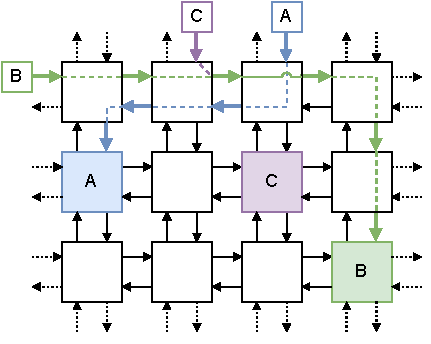
\includegraphics{images/diagrams/dor.drawio.pdf}
    \caption[Ejemplo de funcionamiento del algoritmo de encaminamiento en orden dimensional]{Ejemplo de funcionamiento de DOR con prioridad vertical. Los dispositivos con fondo blanco emiten información a los nodos de fondo coloreado con la misma etiqueta. Debido a que las rutas \textbf{B} y \textbf{C} requieren de un mismo enlace, es imposible que tanto \textbf{B} como \textbf{C} lleguen a su destino. Aunque existen otros caminos mínimos disponibles, DOR no es capaz de aprovecharlos por ser un algoritmo determinista.}
    \label{fig:dimensional_order_routing}
\end{figure}

En un caso concreto en el que la coordenada $(0,0)$ esté arriba a la izquierda (esquina noroeste), y con direccionamiento \textit{absoluto}, podríamos implementarlo siguiendo el siguiente pseudocódigo:

\begin{minted}{python}
def dimensional_order_routing(node_x, node_y, dst_x, dst_y) -> dir:
  if dst_y > node_y:
    return EAST
  elif dst_y < node_y:
    return WEST
  else: # dst_y == node_y
    if dst_x > node_x:
      return SOUTH
    elif dst_x < node_x:
      return NORTH
    else: # (dst_x, dst_y) == (node_x, node_y)
      return LOCAL
\end{minted}

\subsubsection{Evitación de deadlocks}

Una función determinista está libre de deadlocks si y solo si no hay ciclos en su grafo de dependencias~\cite{Duato03}. En el caso de las mallas, estos ciclos solo pueden producirse si se realizan cuatro giros en el mismo sentido (horario o antihorario), por lo que prohibiendo uno de los cuatro giros posibles, tanto horario como antihorario, el algoritmo estaría libre de deadlocks.

En el caso de DOR con prioridad vertical, se lleva a cabo un giro únicamente cuando hemos llegado a la $x$ deseada, por lo que solo se harán giros en los que se cambie la dirección de horizontal a vertical, eliminando la mitad de los giros potenciales y la posibilidad de ocurrir un interbloqueo.
